%! TEX root = diss.tex
\documentclass[../diss.tex]{subfiles}
\chapter{Evaluation}

% ** Other points **
% All unit tests passed (screenshot)
% Some points to show:
% * Exploits parallelism for simulation (was close to 800% CPU usage when `htop`)
% * Very expressive interface, and also raised exceptions like ..., when misused,
%   made development of parallel algorithm a lot easier
% * Extension: Generalized FoxOtto, ran on the same tests, and still produce
%   correct results (unit tests again)
% * Extension: MIMD timing simulation, unit tests
% * Extension: Graph compression, also not just mapped queries to reduced graph and give
%     path length, but also reconstruct list of nodes in original graph.
%     Reference figure as an example
% * Paragraph discussing main plot... TODO: what to say about this?
% * The whole thing about mapping onto real-hardware to do sensitivity analysis
% * Asymptotic complexity of algorithm

% Parallel MatSquare:
% * This section should cover the first 3 points above, quoting them as well...
% * Can have subsections as appropirate
% * squeeze in graph compression somewhere here?
% Parallel MatSquare {{{
\section{Parallel MatSquare}%
\label{sec:Parallel MatSquare}

\begin{wrapfigure}{r}{0.5\textwidth}
    \vspace{-20pt}
    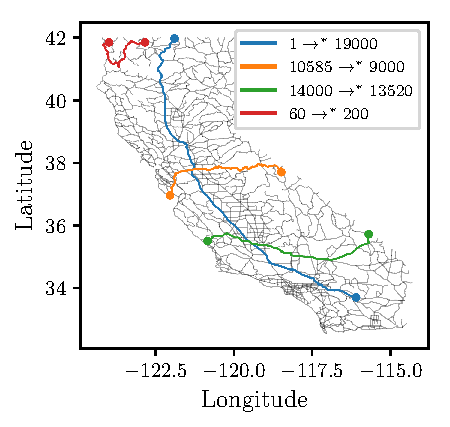
\includegraphics[scale=1]{figs/cal-node-paths.pdf}
    \caption{Four example shortest-paths in the Californian road network
        ($|V|=21048$, $|E|=21693$). These paths consist of
        575, 328, 272, and 207 nodes, respectively.
        % TODO next: Git commits, explain that make diagram, add all diagrams
        %    to GitHub as backup.
    }%
    \label{fig:cal-node-paths}%
    \vspace{-10pt}
\end{wrapfigure}

% (1) MatMul-based algo, find shortet path, can give list of nodes
%  * Manualled created resulted for some set of example graphs (see appendix)
%  * Also implemented serial dijkstra routine that is simple to prove
%    correctness of, and compared the result on $362^2$ possible pair paths on a
%    random large graph, as a unit test. Gives same results
%  * Show example list of nodes, and can make a simple plot on the California
%    road network, on compressed graph, showing a long path...
Introduction. I successfully implemented the \ac{MatSquare} algorithm. To test
the correctness, I set up several unit tests using small graphs where I
manually set up the model answer. See ...  I initially set out to
``\textit{[implement] an algorithm based on matrix multiplication that can find
the length of the shortest path between all pairs of nodes in a graph, and it
is able to give the list of nodes that make up such paths.}'' This resulted in
the \ac{MatSquare} algorithm, which is indeed based on matrix multiplication,
as shown in lines 7--8 in \ref{alg:matsquare}. To assert the correctness of the
path lengths and the path reconstruction, I manually computed the results for
two small graphs, then compared it with the algorithm's output.  Additionally,
I took a subsection of one of the real-world graph datasets\footnote{I used the
    \texttt{graph-extractor.py} script to extract all the nodes and vertices
    within a fixed distance away from a point in the centre of a city in the
Oldenburg city road network dataset. This gave a graph with 430 nodes and 476
edges.}, and tested the path lengths and reconstructions on all $|V|^2$ pairs.
To do this, I implemented Dijkstra's algorithm with path reconstruction, which
is a lot easier to prove the correctness of compared to the \ac{MatSquare}
algorithm. I then ran this and my algorithm and asserted the equality of the
results for all vertex-pairs. This was done in a unit test for reproducibility,
and was done for both the regular and generalised version of the algorithm.

I also successfully extended the project with the graph compression optimisation.
Arbitrary undirected graphs can be compressed through removal of two-degree nodes,
which I have tested by comparing the output to manually-compressed graphs for
some example graphs. The algorithm for mapping \ac{APSP} queries to the compressed
graphs and mapping the results back also work. I tested this by running the
\ac{MatSquare} algorithm on the compressed graph and comparing the distances
found as well as the list of vertices making up the paths, with an \ac{APSP}
algorithm running on the uncompressed graph. This gave the same results for
all $|V|^2$ pairs on a large graph with more than 400 nodes. To further
demonstrate that paths are reconstructed properly when mapping results from
the compressed graph to the uncompressed one, I ran four example queries on the
Californian road network and plotted the list of vertices returned in
\autoref{fig:cal-node-paths}, using additional data about each vertex's
geographical position. Solving \ac{APSP} on such a large graph would also be
infeasible to do in a short amount of time were it not for the graph compression
optimisation.

% (3) Routine minimises amount of data movement
%  * FoxOtto technique is used,
%  * Looking at code, we only send over a single interconnect, so all the data
%    is in the right location after moving it only once. This is clearly
%    minimal if we do not have shared memory. Additionally, no congested
%    interconnect as this would throw `....`
%  (? Table with counts for the number of memory movements in total? ?)
I set out to ``\textit{... minimise the amount of data movement between
processing elements, which is done by using techniques such as Fox-Otto's
algorithm}'' in the matrix-multiplication routine of the \ac{MatSquare}
algorithm. The data movement pattern used is based on the technique
\citeauthor{fox} used. As we see in \ref{alg:foxOtto}, this makes all the
\acp{PE} have exactly the data that they need at each computation phase, after
just sending a packet across a single interconnect channel, a point-to-point
link and the row-broadcast highways. This is clearly minimal data movement if
we are not allowed to utilize shared memory and each \ac{PE} do not have
sufficient private memory to store the whole input.

% }}}

% Parallel simulation:
% (2) MatMul routine parallelised, runs on parallel simulation,
%     each PE can send data
%  * Unit tests for this interface, first show interface working
%  * Show `FoxOtto`, `GeneralisedFoxOtto` and corresponding unit tests
%  * Further evidence of correctness is correctness test for paths, The paths
%    found are unlikely to be correct if the matrix mult. routine is faulty
% * Point on parallelism worked well, 800% CPU
% * Turned out very expressive, and useful exception reported back
% Parallel simulation {{{
\section{Parallel simulation}%
\label{sec:Parallel simulation}

The parallel simulation met all the requirements laid out in
\autoref{sec:Requirements analysis}, which results in ``... \textit{a simulated
massively parallel processor, where each processing element can send data to
each other through simulated interconnects.}'' When creating the
\texttt{Manager} and \texttt{TimedManager}, I can configure the number of
\acp{PE} and the interconnect topology, respectively. The \texttt{Worker}
interface for the parallel programmer is very simple, but it had expressive
power beyond what I required. It also cleanly threw useful exceptions such as
\texttt{InconsistentCommunicationChannelUsageException} if the programmer did
not correctly match up \texttt{send}s and \texttt{receive}s. This programmer
interface has been thoroughly tested through unit tests that cover usage much
more complex than the what was needed in \autoref{alg:foxOtto}. The computation
time measures are done with uncertainty in mind to reduce the amount of noise
in the measurements.
% TODO: this sentence be vague
Additionally, a \ac{MIMD} model is used for the communication time, which is more
complicated to implement compared to a na{\"i}ive \ac{SIMD} model, but with
the benefit of giving more realistic measures. Lastly, the simulation runs in
parallel itself by simultaneously executing work subphases. This sped up
simulation a lot, as computing the results for the compressed Californian road
network for instance took about 25 minutes and the CPU was close to 800\% while
doing so, showing the parallisation was successfull.
% TODO: this last sentence a bit fluffy, maybe compared with Serial Dijkstra time
%       ot compute, but in that case would need disclaimer on not built for my
%       system


I also successfully ``\textit{[p]arallelised the matrix multiplication routine
of the [\ac{MatSquare}] algorithm to run on}'' the parallel system simulation.
This is done through my implementation of the \texttt{FoxOtto} and
\texttt{GeneralisedFoxOtto} which use the \texttt{Worker} interface to create
a parallel algorithm where coordination happens through message passing. The
\texttt{Manager} allows intermediate results from each \ac{PE} to be fetched
after each phase, which I used in my unit tests to verify that the distance
product was computed correctly on test matrix inputs. Another justification for
the correctness of the parallel matrix multiplication step is the \ac{APSP}
unit tests. For these, I used the parallel matrix multiplication step instead
of a serial one, and it is unlikely for the shortest paths to be correct if there
are any faults in the parallel distance product subroutine.

% }}}

% Advantage of parallel computation for solving APSP
% (4) High parallel efficiency for solving APSP
%  * Refer back to equation 2.3 in section 2.1 about computation ratio, then
%    refer to the computation ratio plots and say that high parallel efficeincy,
%    above 90% when problem suffcienctly sub-divided
% * Discuss the main plot, and explain sensitivity analysis
% * Explain the first column of plots as well...
% Advantage of parallel computation for solving APSP {{{
\section{Advantage of parallel computation for solving APSP}%
\label{sec:Advantage of parallel computation for solving APSP}

\begin{figure}
    \centering
    \subfigure[Figure A]{%
        \label{fig:main-plot-fig-a}%
        % TODO: fix which plots are there
        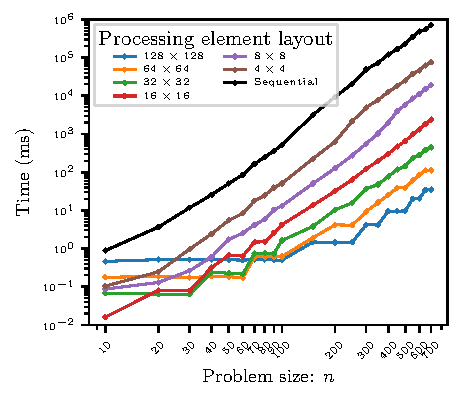
\includegraphics{figs/plots/total-time-scaling-sandy-full-width-no-errorbars.pdf}%
        \hfill%
        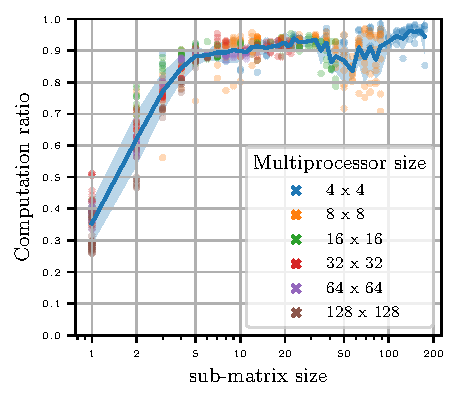
\includegraphics{figs/plots/ratio-bucket-sandy-half-scale.pdf}
    }%
    \vskip\baselineskip\vspace{-25pt}%
    \subfigure[Figure B]{%
        \label{fig:main-plot-fig-b}%
        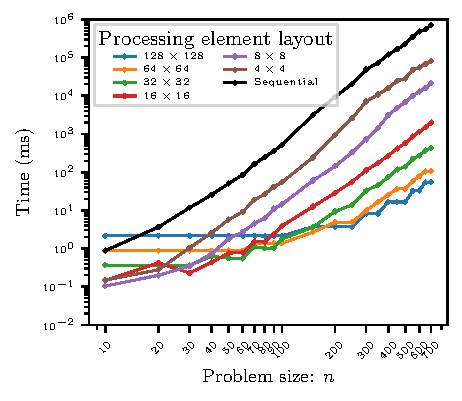
\includegraphics{figs/plots/total-time-scaling-taihu-full-width-no-errorbars.pdf}%
        \hfill%
        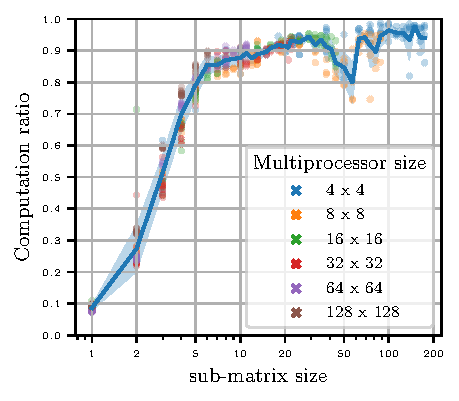
\includegraphics{figs/plots/ratio-bucket-taihu-half-scale.pdf}
    }%
    \vskip\baselineskip\vspace{-25pt}%
    \subfigure[Figure C]{%
        \label{fig:main-plot-fig-c}%
        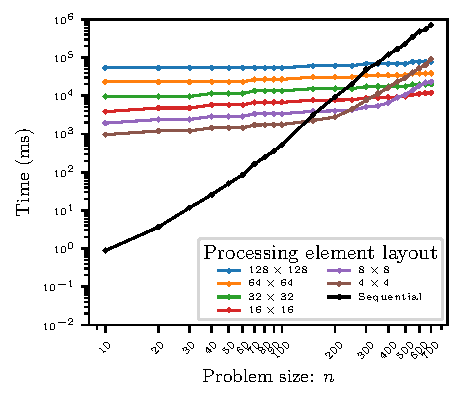
\includegraphics{figs/plots/total-time-scaling-internet-full-width-no-errorbars.pdf}%
        \hfill%
        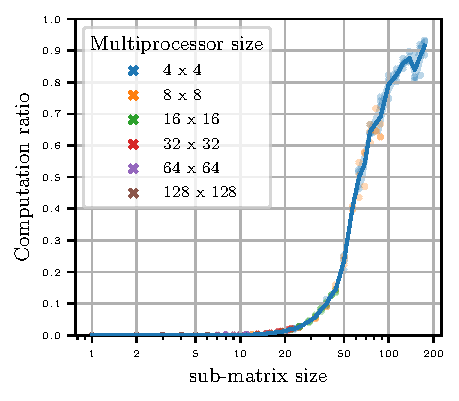
\includegraphics{figs/plots/ratio-bucket-internet-half-scale.pdf}
    }%
    \caption{Global caption that might be a bit long as it goes over two lines, right
        about now... It might even go over three lines since we are daring today. Just
    this extra sentence should do it.}
    \label{fig:main-eval-plot}
\end{figure}

% Introduction tying this section's subs together

% Choice of communication parameters:
% * sensitivity analysis
% * map onto real hardware for more applicable conclusions
% * The three models used and reference

% \begin{wraptable}{r}{0.60\textwidth}
%         \centering
%         \begin{tabular}{|p{0.1\textwidth}|p{0.1\textwidth}|p{0.15\textwidth}|}
%             \hline
%             \textbf{Parallel system} & \textbf{Latency} & \textbf{Bandwidth} \\
%             \hline
%             Multi-core processor & 107 clock cycles & 32 Bytes per cycle \\
%             \hline
%         \end{tabular}%
%         \caption{Caption}%
%         \label{tab:node-paths}%
% \end{wraptable}

% Sandy bridge
\paragraph{Multi-core processor}%
\label{par:Multi-core processor}

The Sandy Bridge microarchitecture supports multiple cores which execute in
\ac{MIMD} fashion, and the L3 cache is shared across all cores while the
lower-level caches are local to each core \cite{sandyBridge}. For one core to
send a data from its private L1 cache to another core's L1 cache,
we must look at the round-trip time of the cache coherence protocol because
the receiving core must message the sending core and it must then wait for
the cache line to come back. \citeauthor{timJones} have done measurements of
this kind of cache coherence latency, and found that for the Sandy Bridge
microarchitecture, the round-trip latency is about 107 80\% of the time. I make
the simplifying assumption that the latency is constantly at 107 cycles, and
this delay is fixed whatever the clock frequency is, as I will be using the
clock frequency of my own laptop \cite{timJones}.
In the ring interconnect used to implement cache coherency in the Sandy Bridge microarchitecture, the data ring used
has a bandwidth of 32 bytes per cycle. I will therefore make the assumption that when sending data from one private
L1 cache to another through the ring interconnect (using cache coherncy protocol), this is the available bandwidth.

Cite these guys: \cite{sandyBridge} and \cite{timJones}.

% Taihu light
\paragraph{Supercomputer}%
\label{par:Supercomputer}

\cite{sunway} this guy.

% Internet
Bandwidth internet values based on report from \url{https://www.cable.co.uk/broadband/speed/worldwide-speed-league/}. Latency values for Europe based on statistics from
Verizon here \url{https://www.verizon.com/business/terms/latency/}. Chose round-trip
time because TCP transfer, and ACKs etc.


% Discuss total time scaling
% * As num. PE *4, we have a decrease in computation time, decrease gets slightly
%   smaller the more low we go, this is for large problem sizes where even out
% * At the start, there are many flat lines, with stepwise increase, this is
%   because of asymptotic complexity, and padding requiered
% * As increase communication constants, serial gets better, but parallel always
%   catches up eventually,

% Discuss parallel efficiency
% * Related parallel computation to efficiency
% * quote success criteria
% * show that for all parameter choices, evenually reach over 90 and even 95\%
%   efficiency


% }}}

\section{Evaluation metrics}

Nothing in this section

\section{Parallel matrix-multiplication}

\newpage
See \autoref{fig:example1} for some example plots. There is also
\autoref{fig:example3} which shows some stuff.


% Example figure
\begin{figure}
    \begin{center}
        % \includegraphics[scale=1]{figs/plots/example1.pdf}
        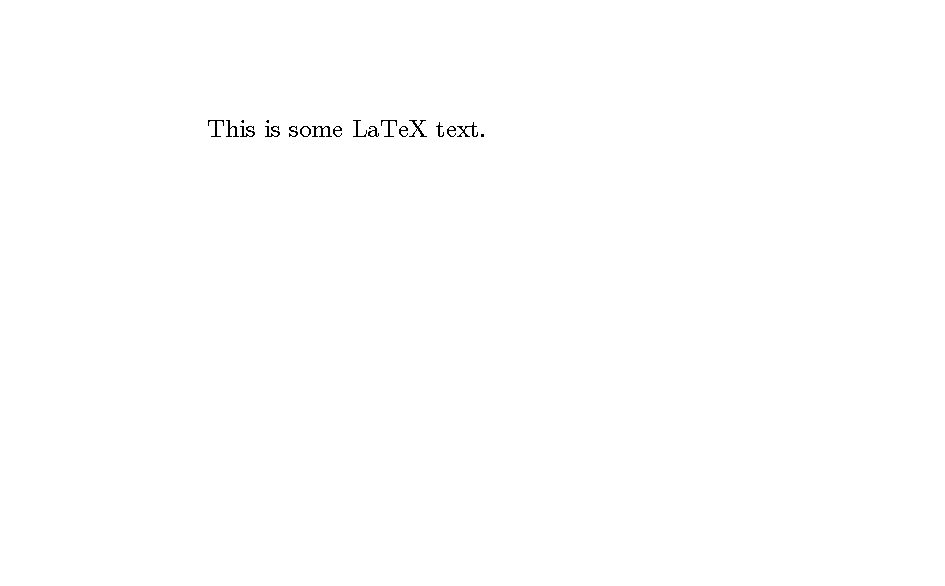
\includegraphics{inkscape-diagrams/template-diagram2.pdf}
    \end{center}
    \caption{Example diagram produced with inkscape}
    \label{fig:example1}
\end{figure}

% Comparison of computation ratio
\begin{figure}%
    \hfill
    \subfigure[Sandy bridge]{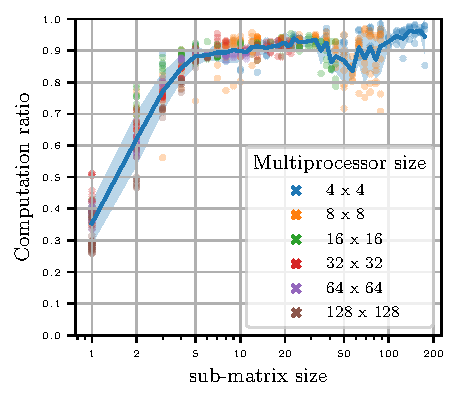
\includegraphics[scale=0.95]{figs/plots/ratio-bucket-sandy-half-scale.pdf}}
    \hfill
    \subfigure[Taihu light]{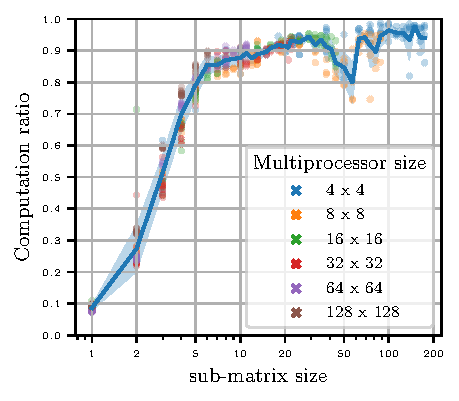
\includegraphics[scale=0.95]{figs/plots/ratio-bucket-taihu-half-scale.pdf}}
    \hfill
    \caption{Title for both, and explain some more...}
    \label{fig:example2}
\end{figure}

% Third example figure
\begin{figure}
    \begin{center}
        % \includegraphics[scale=1]{figs/plots/example3.pdf}
        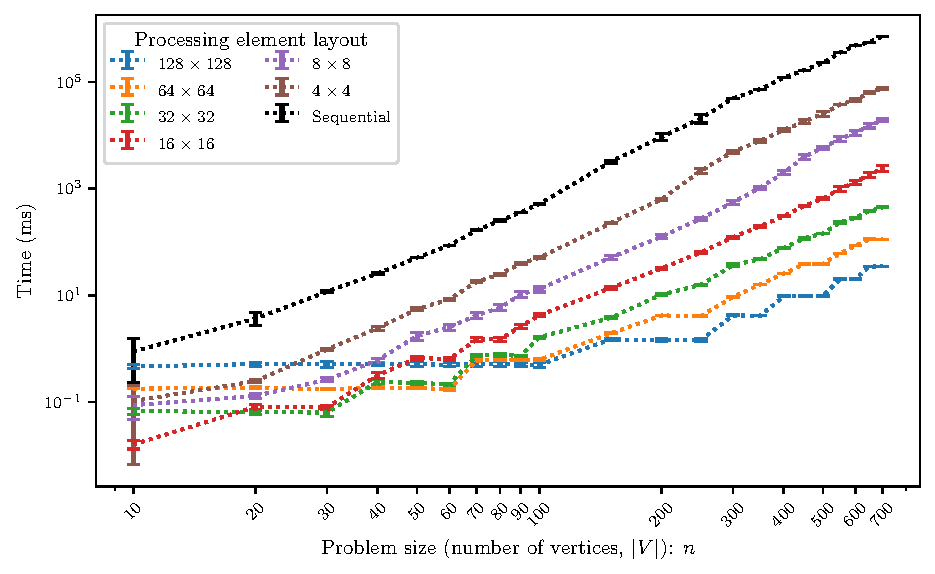
\includegraphics{figs/plots/total-time-scaling-sandy-full-width.pdf}
    \end{center}
    \caption{Sandy bridge total time scaling}
    \label{fig:example3}
\end{figure}

% Fourth example figure
\begin{figure}
    \begin{center}
        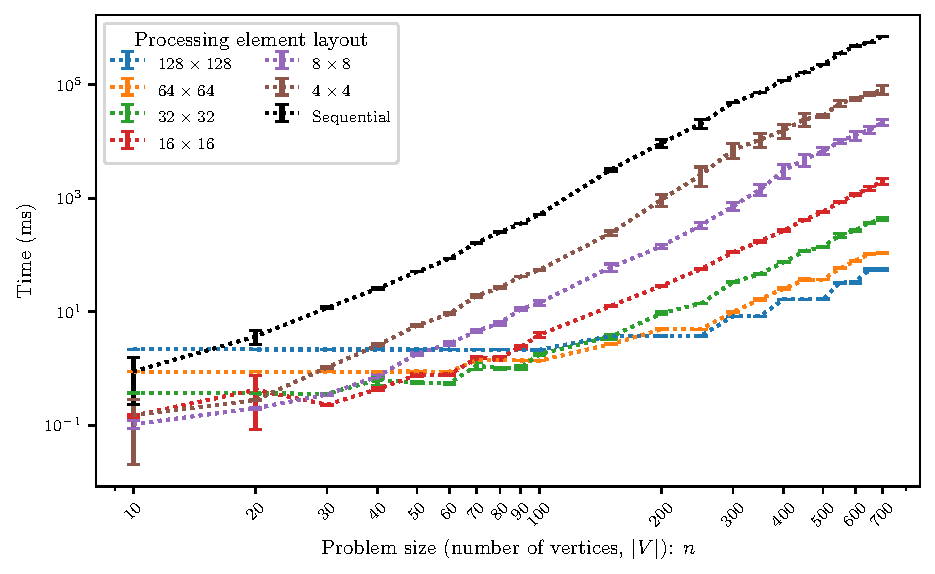
\includegraphics[scale=1]{figs/plots/total-time-scaling-taihu-full-width.pdf}
    \end{center}
    \caption{Taihu light total time scaling}
    \label{fig:example4}
\end{figure}


% Explanation of where constants from:


% vim: foldmethod=marker
